% \section{Distributed spatial processing}
% \label{sec:distributed-spatial-processing}
% Section \ref{background:cloud-native-data-architecture:distributed-and-non-distributed-computation} introduced the trade-off between distributed and non-distributed compute, and Section \ref{background:spatial-data-formats-and-storage-models:full-database-engines} described PostGIS and DuckDB as full single-node engines. This section turns to the third architectural class compared in this thesis: distributed spatial processing on a cluster of executors that share neither memory nor local disk. The aim is to make precise where time and cost are spent when a spatial query runs on a Spark-based engine, so that observed differences against PostGIS and DuckDB can be attributed to specific mechanisms rather than to the label \enquote{distributed}. Section \ref{background:distributed-spatial-processing:the-lifecycle-of-a-distributed-spatial-query} traces a query through the engine and names the stages that account for wall-clock time. Section \ref{background:distributed-spatial-processing:spatial-partitioning-and-parallel-efficiency} identifies spatial partitioning as the lever that decides whether the lifecycle parallelizes. Section \ref{background:distributed-spatial-processing:distributed-spatial-operations} reviews the dominant operations on this lifecycle, and Sections \ref{background:distributed-spatial-processing:apache-sedona} and \ref{background:distributed-spatial-processing:databricks-as-a-sedona-run-time} describe the concrete implementations evaluated in this thesis.

\section{Distributed spatial processing}
\label{background:distributed-spatial-processing}
Section \ref{background:cloud-native-data-architecture:distributed-and-non-distributed-computation} introduced the trade-off between distributed and non-distributed compute, and Section \ref{background:spatial-data-formats-and-storage-models:full-database-engines} described PostGIS and DuckDB as full single-node engines. This section turns to the third architectural class compared in this thesis: distributed spatial processing on a shared-nothing cluster, in which executors share neither memory nor local disk. The aim is to specify where time and cost are spent when a spatial query runs on an engine built on Apache Spark, a general-purpose cluster-computing framework for in-memory distributed processing. Observed differences against PostGIS and DuckDB can then be attributed to specific mechanisms rather than to the label \enquote{distributed}. Section \ref{background:distributed-spatial-processing:the-lifecycle-of-a-distributed-spatial-query} traces a query through the engine and names the stages that account for wall-clock time, the elapsed time from query submission to result return. Section \ref{background:distributed-spatial-processing:spatial-partitioning-and-parallel-efficiency} identifies spatial partitioning as the lever that decides whether the lifecycle parallelizes. Section \ref{background:distributed-spatial-processing:distributed-spatial-operations} reviews the dominant operations on this lifecycle, and Sections \ref{background:distributed-spatial-processing:apache-sedona} and \ref{background:distributed-spatial-processing:databricks-as-a-sedona-run-time} describe the concrete implementations evaluated in this thesis.

% \subsection{The lifecycle of a distributed spatial query}
% \label{subsec:lifecycle}
% A query submitted to a Spark-based engine such as Apache Sedona is first planned on a single coordinator process, the \emph{driver}, which uses the Catalyst optimizer to translate the \acrshort{sql} or DataFrame input into a physical plan that the cluster will execute \parencite{armbrust2015_spark_sql_relational_data_processing, spark2024_cluster_mode_overview}. This planning phase runs sequentially before any task is dispatched, and on workloads with short execution times, it is part of the fixed overhead that does not shrink with additional workers.

% The physical plan executes against an underlying abstraction of partitioned, fault-tolerant collections. The \acrfull{rdd} is a \enquote{distributed memory abstraction that lets programmers perform in-memory computations on large clusters in a fault-tolerant manner} \parencite{zaharia2012_resilient_distributed_datasets}. DataFrames in Spark \acrshort{sql} compile down to \acrshort{rdd} operations after Catalyst's physical planning phase \parencite{armbrust2015_spark_sql_relational_data_processing}. The driver translates the physical plan into a \acrfull{dag} of \emph{stages}, each consisting of \emph{tasks} that run in parallel on \emph{executors}, the \acrshort{jvm} processes that hold cached partitions and execute task code \parencite{zaharia2012_resilient_distributed_datasets, spark2024_cluster_mode_overview}.

% Within a stage, transformations run locally on each executor \parencite{zaharia2012_resilient_distributed_datasets}. Operations that require records from many partitions trigger a \emph{shuffle}, which writes intermediate data to local disk and fetches it across the network in the next stage \parencite{zaharia2012_resilient_distributed_datasets, spark2024_job_scheduling}. Shuffles transfer data between executors and are a major source of network traffic during a query, and the volume of bytes they move, the \emph{shuffle volume}, affects both elapsed time and bytes received.

% Two phases of this lifecycle are worth naming. The \emph{executor read time} is the time spent reading input partitions from storage at the start of the query, and is dominated by network round-trips when the data lives in Azure object storage rather than on local disk. \emph{Driver collection} is the time spent at the end of the query returning results to the driver via an action such as \texttt{collect}, and is sequential in the size of the result set \parencite{zaharia2012_resilient_distributed_datasets}. Figure \ref{fig:distributed-spatial-query-lifecycle} situates both phases within the full lifecycle.

% \begin{figure}[H]
% 	\centering
% 	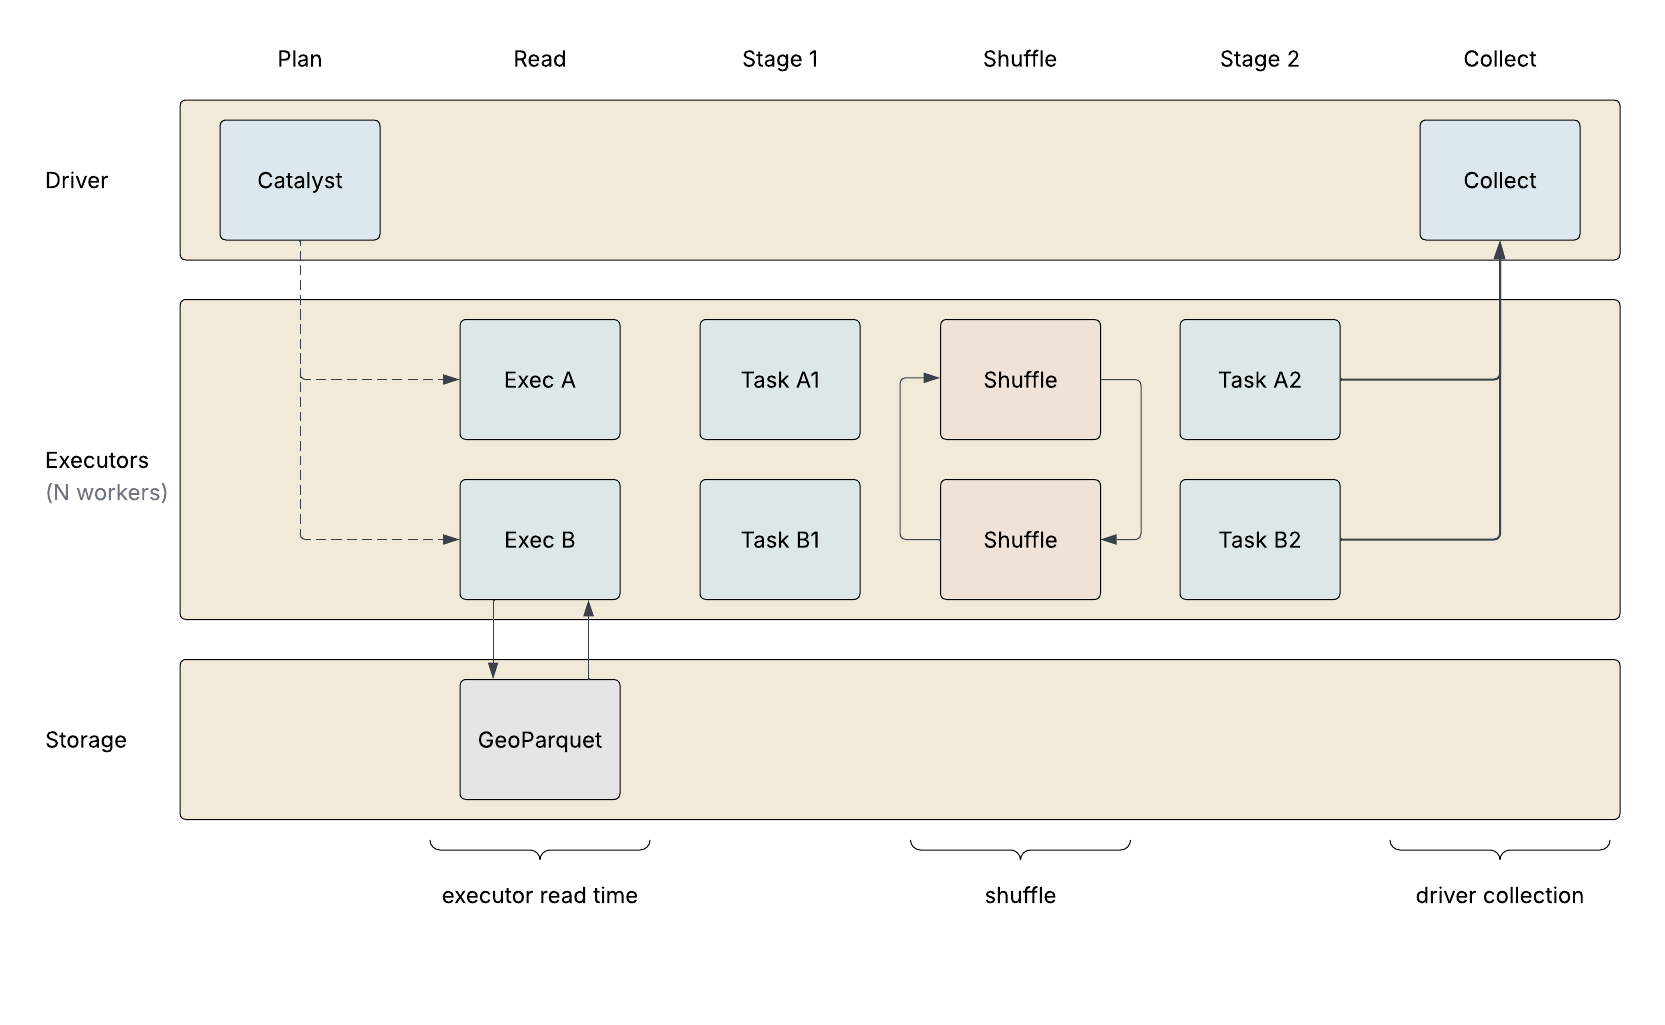
\includegraphics[width=0.8\textwidth]{Chapters/02-background/sub-chapters/figures/02-distributed-spatial-query-lifecycle.png}
% 	\caption[Lifecycle of a distributed spatial query]{Lifecycle of a distributed spatial query on a Spark-based engine, shown as a swimlane across the driver, executors, and object storage. The six columns trace the query from planning, through reading input partitions, two narrow stages separated by a shuffle, and final result collection. The brackets below the storage lane mark the three named phases referenced in the prose: \emph{executor read time}, \emph{shuffle}, and \emph{driver collection}. Inter-lane arrows distinguish the network channels. The dashed gray arrows from Catalyst to each executor carry the serialized plan and task descriptors at a small, input-independent cost. The arrows between the executors and storage carry the data reads, with volume scaling with input size. The coral arrows around the shuffle column carry intra-cluster traffic between executors as Stage~1 outputs are redistributed for Stage~2. The arrows from the Stage~2 tasks to Collect carry the result set back to the driver, with volume scaling with its size.}
%  	\label{fig:distributed-spatial-query-lifecycle}
% \end{figure}

% The lifecycle also determines how bytes are exchanged across the system, which the benchmark measures directly. Three channels carry the bulk of network traffic. The driver-to-executor channel carries the serialized plan and task descriptors, a small and largely fixed cost independent of input size \parencite{spark2024_cluster_mode_overview}. The executor-to-storage channel carries the actual data reads from object storage and scales with the input size and the number of files not pruned by metadata. The executor-to-driver channel at the end of the query carries either the full result set, when the query ends in an action that collects rows, or only a small aggregate such as a row count, when the query ends in a write or a count action \parencite{zaharia2012_resilient_distributed_datasets}. The total bytes transferred reported by the benchmark is the sum of these three channels, and the relative split among them is one of the signals available to attribute observed performance to specific parts of the lifecycle.

\subsection{The lifecycle of a distributed spatial query}
\label{background:distributed-spatial-processing:the-lifecycle-of-a-distributed-spatial-query}
A query submitted to a Spark-based engine such as Apache Sedona is first planned on a single coordinator process, the driver, which uses the Catalyst optimizer, Spark's query planner, to translate the \acrshort{sql} or DataFrame input into a physical plan, the concrete sequence of operations the cluster will execute \parencite{armbrust2015_spark_sql_relational_data_processing, spark2024_cluster_mode_overview}. A DataFrame is Spark's tabular abstraction over a distributed collection of rows, comparable in shape to a relational table \parencite{armbrust2015_spark_sql_relational_data_processing}. Planning runs sequentially before any task is dispatched, so on workloads with short execution times it constitutes fixed overhead that does not shrink with additional workers.

The physical plan executes against an underlying abstraction of partitioned, fault-tolerant collections. The \acrfull{rdd} is a \enquote{distributed memory abstraction that lets programmers perform in-memory computations on large clusters in a fault-tolerant manner} \parencite{zaharia2012_resilient_distributed_datasets}. DataFrames in Spark \acrshort{sql}, Spark's relational query module, compile down to \acrshort{rdd} operations after Catalyst's physical planning phase \parencite{armbrust2015_spark_sql_relational_data_processing}. The driver translates the physical plan into a \acrfull{dag} of \emph{stages}, each consisting of \emph{tasks} that run in parallel on \emph{executors}, the \acrfull{jvm} processes that hold cached partitions and execute task code \parencite{zaharia2012_resilient_distributed_datasets, spark2024_cluster_mode_overview}. The \acrshort{jvm} is the Java runtime that hosts Spark code on each worker.

Within a stage, transformations run locally on each executor, where a transformation is a lazy operation such as filter or map that describes a new dataset rather than producing one immediately \parencite{zaharia2012_resilient_distributed_datasets}. Operations that require records from many partitions trigger a \emph{shuffle}, which writes intermediate data to local disk and fetches it across the network in the next stage \parencite{zaharia2012_resilient_distributed_datasets, spark2024_job_scheduling}. Shuffles transfer data between executors and are a major source of network traffic during a query, and the volume of bytes they move, the \emph{shuffle volume}, affects both elapsed time and bytes received.

Two phases of this lifecycle are worth naming. The \emph{executor read time} is the time spent reading input partitions from storage at the start of the query, dominated by network round-trips when the data lives in Azure object storage rather than on local disk. \emph{Driver collection} is the time spent at the end of the query returning results to the driver via an action such as \texttt{collect}; an action is the operation that forces accumulated transformations to execute, and the phase itself is sequential in the size of the result set \parencite{zaharia2012_resilient_distributed_datasets}. Figure \ref{fig:distributed-spatial-query-lifecycle} situates both phases within the full lifecycle.

\begin{figure}[H]
	\centering
	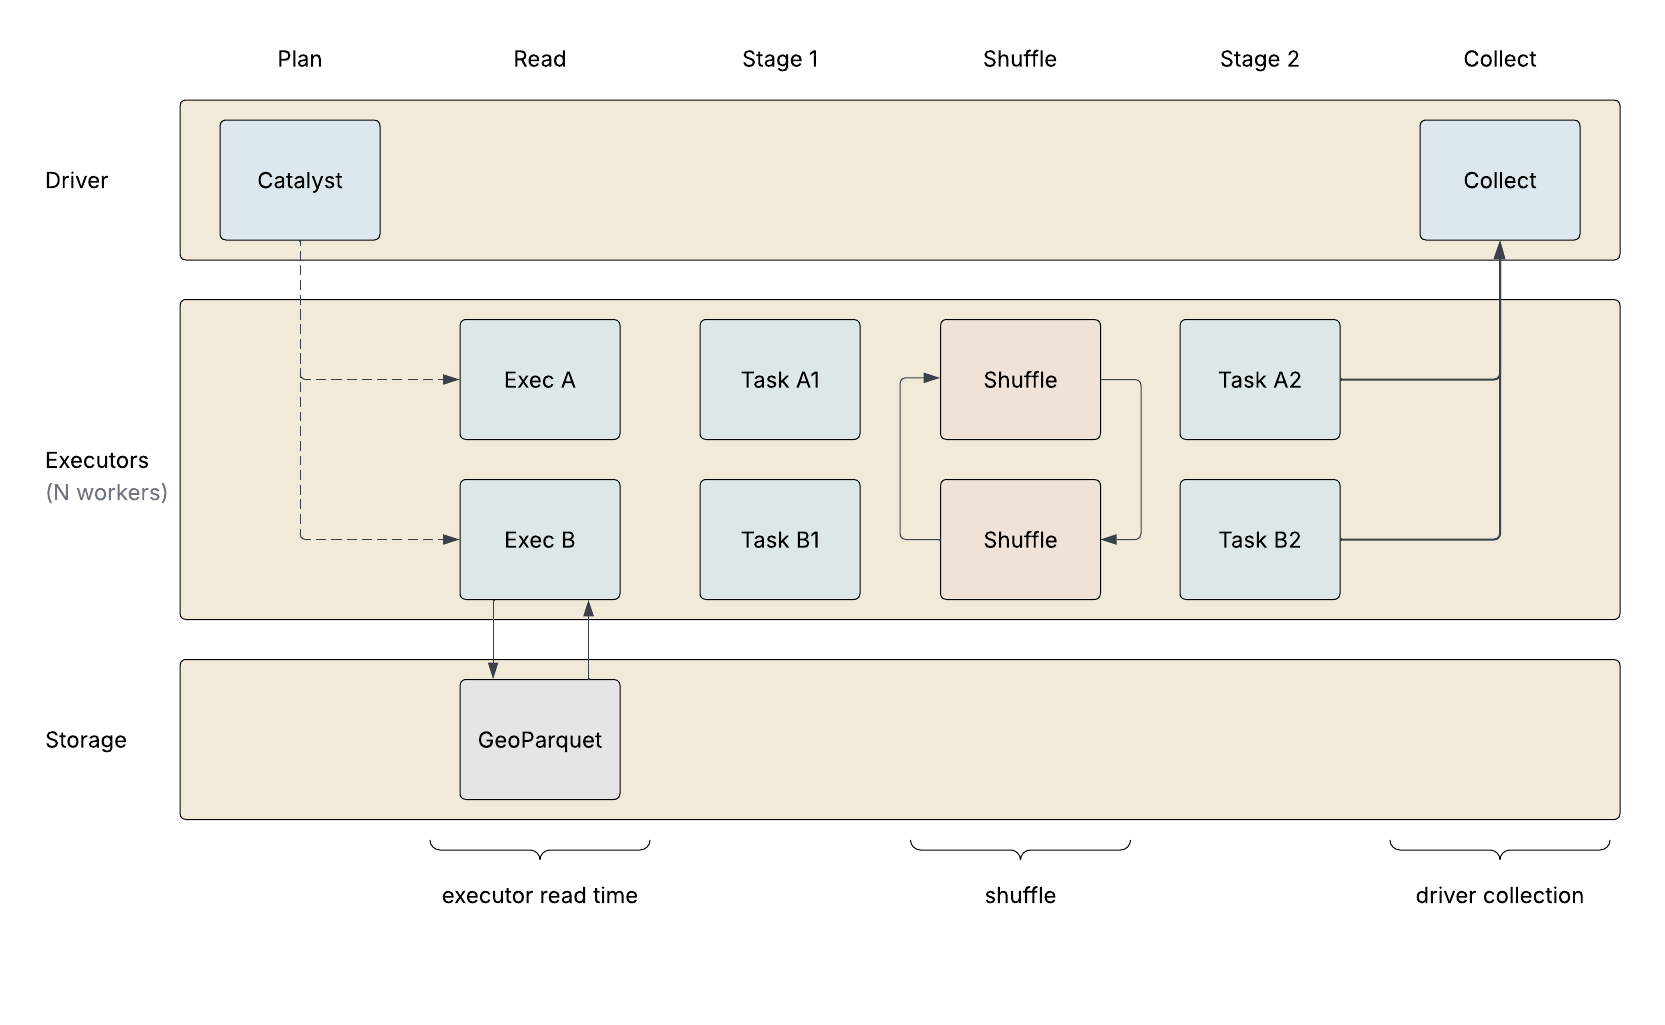
\includegraphics[width=0.8\textwidth]{Chapters/02-background/sub-chapters/figures/02-distributed-spatial-query-lifecycle.png}
	\caption[Lifecycle of a distributed spatial query]{Lifecycle of a distributed spatial query on a Spark-based engine, shown as a swimlane across the driver, executors, and object storage. The six columns trace the query from planning, through reading input partitions, two narrow stages separated by a shuffle, and final result collection. The brackets below the storage lane mark the three named phases referenced in the prose: \emph{executor read time}, \emph{shuffle}, and \emph{driver collection}. Inter-lane arrows distinguish the network channels. The dashed gray arrows from Catalyst to each executor carry the serialized plan and task descriptors at a small, input-independent cost. The arrows between the executors and storage carry the data reads, with volume scaling with input size. The coral arrows around the shuffle column carry intra-cluster traffic between executors as Stage~1 outputs are redistributed for Stage~2. The arrows from the Stage~2 tasks to Collect carry the result set back to the driver, with volume scaling with its size.}
 	\label{fig:distributed-spatial-query-lifecycle}
\end{figure}

The lifecycle also determines how bytes are exchanged across the system, which the benchmark measures directly. Three channels carry the bulk of network traffic. The driver-to-executor channel carries the serialized plan and task descriptors, a small and largely fixed cost independent of input size \parencite{spark2024_cluster_mode_overview}. The executor-to-storage channel carries the actual data reads from object storage and scales with the input size and the number of files not pruned by metadata. The executor-to-driver channel at the end of the query carries either the full result set, when the query ends in an action that collects rows, or only a small aggregate such as a row count, when the query ends in a write or a count action \parencite{zaharia2012_resilient_distributed_datasets}. The total bytes transferred reported by the benchmark is the sum of these three channels, and the relative split among them is one of the signals available for attributing observed performance to specific parts of the lifecycle.

% \subsection{Spatial partitioning and parallel efficiency}
% \label{subsec:partitioning}
% The lifecycle parallelizes only if the input is split into roughly equal pieces of work that executors can process independently. The mechanism that does this splitting is a \emph{partitioner}, a function that assigns each input record to one of several partitions, each of which becomes a unit of work for an executor \parencite{spark2024_partitioner_api, zaharia2012_resilient_distributed_datasets}. Spark's built-in partitioners, hash and range, distribute records by hashing or sorting their keys \parencite{spark2024_partitioner_api}. Neither method considers the geometry of the records. Two polygons that share a boundary will typically land on different partitions under a hash partitioner, and any operation whose semantics depend on geometry therefore has to either compare every record against every other or repartition the data spatially before it can run efficiently, the latter being the approach taken by spatial extensions to Spark \parencite{yu2019_geospark_perspective_beyond}. Figure \ref{fig:hash-vs-spatial-partitioning} contrasts the two on the same set of features.
% 
% \begin{figure}[H]
% 	\centering
% 	\subfloat[Hash partitioning.\label{fig:hash-partitioning}]{%
% 		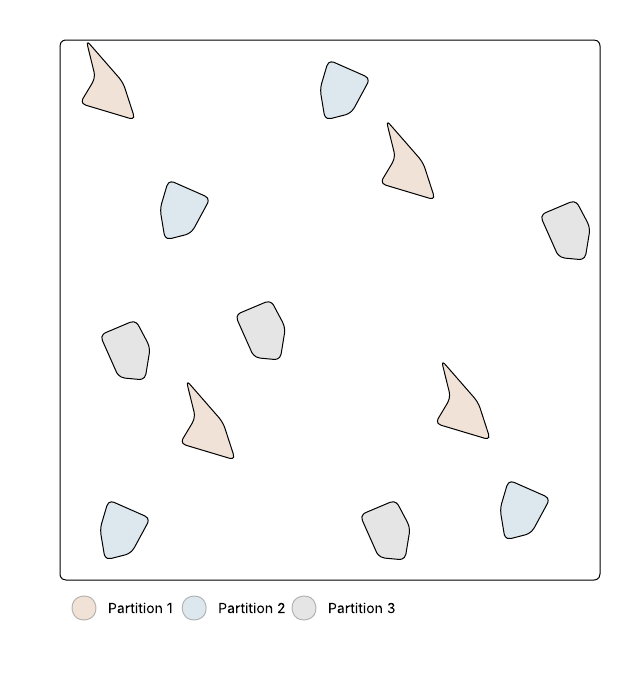
\includegraphics[valign=t, width=0.45\textwidth]{Chapters/02-background/sub-chapters/figures/02-hash-partitioning.png}%
% 	}
% 	\hfill
% 	\subfloat[Spatial partitioning.\label{fig:geographic-partitioning}]{%
% 		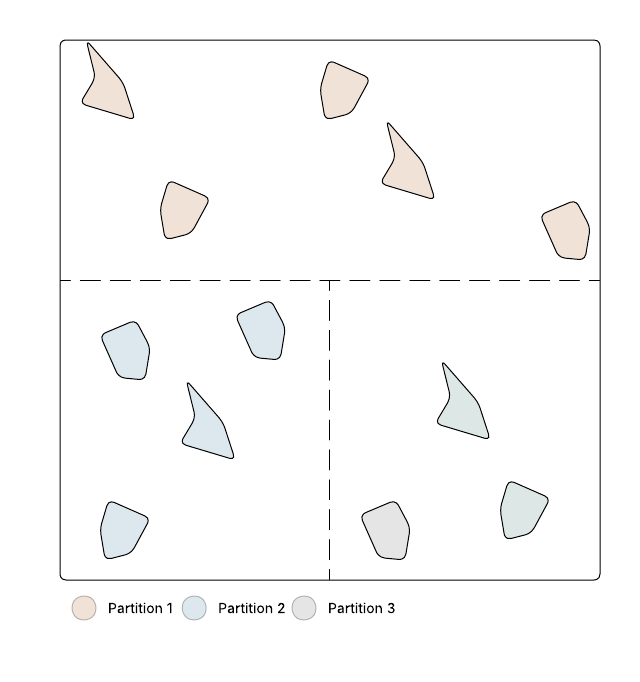
\includegraphics[valign=t, width=0.45\textwidth]{Chapters/02-background/sub-chapters/figures/02-geographic-partitioning.png}%
% 	}
% 	\caption[Hash versus spatial partitioning of the same features]{Hash versus spatial partitioning of the same set of features. Both panels show the same polygons in identical positions; color encodes partition assignment, with each color corresponding to one partition handled by a different executor. (a) Under hash partitioning, color is uncorrelated with position, so polygons that share a boundary in the plane typically land on different partitions. (b) Under spatial partitioning, the study area is divided into spatially contiguous cells (dashed dividers) and all polygons within a cell share a color, so locality in the plane is preserved as locality in partition assignment. Adapted from \parencite{eldawy2015_spatial_partitioning_techniques}.}
% 	\label{fig:hash-vs-spatial-partitioning}
% \end{figure}
% 
% Spatial partitioners replace this with a function of the geometry's location and extent. \textcite{yu2019_geospark_perspective_beyond} describes four such partitioners that have become standard in the Spark ecosystem: \enquote{uniform grid, R-tree, Quad-Tree, and KDB-Tree}. A uniform grid divides the study area into equal cells and is the cheapest to compute, but is sensitive to data density. The tree-based partitioners are constructed from a sample of the input so that each leaf cell contains a similar number of records, which yields more balanced partition sizes when the underlying distribution is skewed \parencite{yu2019_geospark_perspective_beyond}. After the global partitioner assigns records to partitions, each partition can build a local in-memory index, typically an R-tree or Quad-Tree, that accelerates per-partition processing \parencite{yu2019_geospark_perspective_beyond}. This two-tier design mirrors the partition-then-search structure of single-node spatial indexes such as the R-tree \parencite{guttman1984_rtree_dynamic_index}, applied here at the cluster scale.
% 
% Even with a spatial partitioner, work can still be distributed unevenly because the data, the query workload, or both are skewed. \textcite{tang2020_locationspark_distributed_spatial_query} term this failure mode \enquote{spatial query skew} and observe that traditional spatial partitioners balance data across cells but not the query load. The consequence they identify is that if many query windows fall inside one cell, the executor holding that cell becomes a straggler regardless of how evenly the records were distributed. The realized parallelism of the job is therefore bounded above by the most loaded partition: if a workload distributes evenly across $n$ executors, run-time falls roughly as $1/n$ until coordination cost dominates, but if a single partition holds half the join output, no number of additional executors will reduce run-time below the time taken to process that partition. Skew is a well-recognized cause of poor scaling in distributed query systems \parencite{kwon2012_skewtune_mitigating_skew}, and a likely explanation when a distributed engine fails to scale even though the work appears to decompose cleanly across executors.

\subsection{Spatial partitioning and parallel efficiency}
\label{background:distributed-spatial-processing:spatial-partitioning-and-parallel-efficiency}
The lifecycle parallelizes only when the input is split into pieces of roughly equal work that executors can process independently. This splitting is performed by a \emph{partitioner}, a function that assigns each input record to one of several partitions, each of which becomes a unit of work for an executor \parencite{spark2024_partitioner_api, zaharia2012_resilient_distributed_datasets}. Spark's built-in partitioners, hash and range, distribute records by hashing or sorting their keys, with no consideration of the geometry attached to each record \parencite{spark2024_partitioner_api}. Two polygons that share a boundary in the plane will typically land on different partitions under a hash partitioner, so any operation whose semantics depend on geometry must either compare every record against every other or repartition the data spatially before it can run efficiently. Spatial extensions to Spark take the latter route \parencite{yu2019_geospark_perspective_beyond}. Figure \ref{fig:hash-vs-spatial-partitioning} contrasts the two on the same set of features.

\begin{figure}[H]
	\centering
	\subfloat[Hash partitioning.\label{fig:hash-partitioning}]{%
		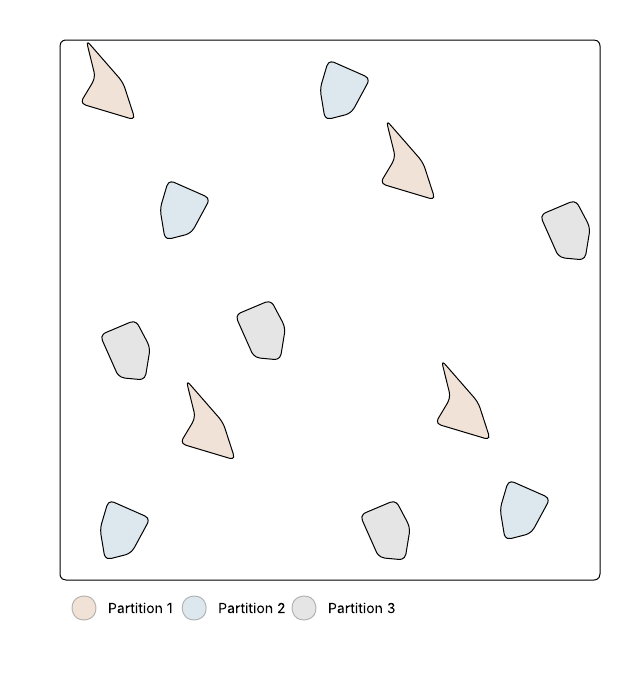
\includegraphics[valign=t, width=0.45\textwidth]{Chapters/02-background/sub-chapters/figures/02-hash-partitioning.png}%
	}
	\hfill
	\subfloat[Spatial partitioning.\label{fig:geographic-partitioning}]{%
		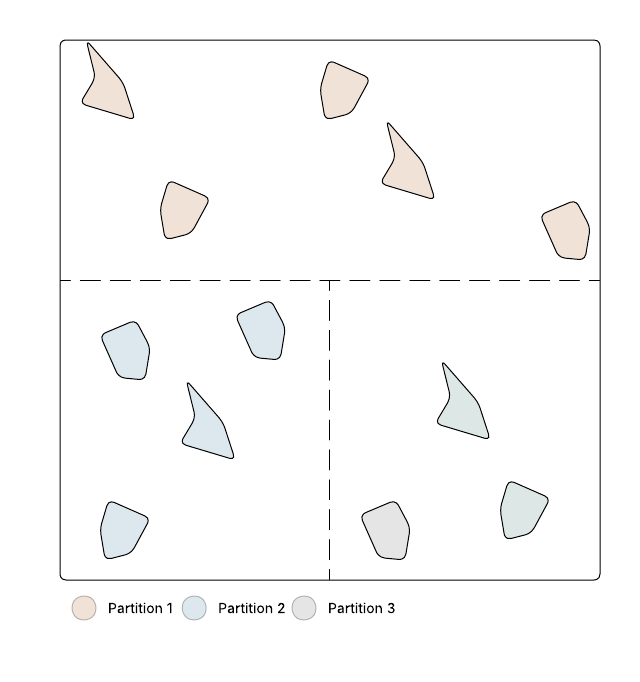
\includegraphics[valign=t, width=0.45\textwidth]{Chapters/02-background/sub-chapters/figures/02-geographic-partitioning.png}%
	}
	\caption[Hash versus spatial partitioning of the same features]{Hash versus spatial partitioning of the same set of features. Both panels show the same polygons in identical positions; color encodes partition assignment, with each color corresponding to one partition handled by a different executor. (a) Under hash partitioning, color is uncorrelated with position, so polygons that share a boundary in the plane typically land on different partitions. (b) Under spatial partitioning, the study area is divided into spatially contiguous cells (dashed dividers) and all polygons within a cell share a color, so locality in the plane is preserved as locality in partition assignment. Adapted from \parencite{eldawy2015_spatial_partitioning_techniques}.}
	\label{fig:hash-vs-spatial-partitioning}
\end{figure}

Spatial partitioners replace this key-based assignment with a function of each geometry's location and extent. \textcite{yu2019_geospark_perspective_beyond} describes four such partitioners that have become standard in the Spark ecosystem: \enquote{uniform grid, R-tree, Quad-Tree, and KDB-Tree}. A uniform grid divides the study area into equal cells and is the cheapest to compute, but it is sensitive to data density. The tree-based partitioners are constructed from a sample of the input so that each leaf cell contains a similar number of records, which yields more balanced partition sizes on skewed distributions \parencite{yu2019_geospark_perspective_beyond}. Once the global partitioner has assigned records to partitions, each partition can build a local in-memory index, typically an R-tree or Quad-Tree, that accelerates per-partition processing \parencite{yu2019_geospark_perspective_beyond}. This two-tier design mirrors the partition-then-search structure of single-node spatial indexes such as the R-tree \parencite{guttman1984_rtree_dynamic_index}, applied here at the cluster scale.

A spatial partitioner does not by itself guarantee even work distribution: the data, the query workload, or both may still be skewed. \textcite{tang2020_locationspark_distributed_spatial_query} term this failure mode \enquote{spatial query skew} and observe that traditional spatial partitioners balance data across cells but not query load. The consequence they identify is that when many query windows fall inside one cell, the executor holding that cell becomes a straggler, the single slow worker whose unfinished tasks hold up the rest of the stage, regardless of how evenly the records were distributed. The realized parallelism of the job, the speedup actually obtained as workers are added, is therefore bounded above by the most loaded partition: if a workload distributes evenly across $n$ executors, run-time falls roughly as $1/n$ until coordination cost dominates, but if a single partition holds half the join output, no number of additional executors will reduce run-time below the time taken to process that partition. Skew is a well-recognized cause of poor scaling in distributed query systems \parencite{kwon2012_skewtune_mitigating_skew}, and a likely explanation when a distributed engine fails to scale even though the work appears to decompose cleanly across executors.

% \subsection{Distributed spatial operations}
% \label{subsec:dist-operations}
% This subsection describes two spatial operations: the spatial range query, which filters one input against a fixed query window, and the spatial join, which evaluates a spatial predicate between two inputs. They differ sharply in how they exercise the lifecycle described in Section \ref{background:distributed-spatial-processing:the-lifecycle-of-a-distributed-spatial-query}.

% A spatial range query returns all geometries from an input that lie within a fixed query window \parencite{yu2019_geospark_perspective_beyond}. It runs entirely within a single stage: each partition filters its own contents independently without coordination with other executors \parencite{yu2019_geospark_perspective_beyond}. Any optimization that reduces the number of partitions scanned, therefore translates directly into run-time improvement. File-level bounding-box metadata in GeoParquet is one such optimization, as it allows the engine to skip files whose extent does not overlap the query window \parencite{sedona2024_geoparquet_loader}. A range query is the operation in which a distributed engine is hardest to distinguish from a single-node engine reading the same files, because the work naturally decomposes across files, regardless of the partitioner.

% The spatial join is the operation where the distribution either pays off or breaks down. A spatial join combines two inputs using a spatial predicate, such as intersection or distance, returning the records from each input that satisfy it \parencite{yu2019_geospark_perspective_beyond}. Because records from different executors must be brought together for comparison, the join is a wide operation that crosses a stage boundary \parencite{yu2019_geospark_perspective_beyond}, and two execution strategies have emerged to handle it. In a \emph{broadcast} join, the smaller input is shipped to every partition of the larger input, and each executor then performs a local join against its own partition \parencite{yu2019_geospark_perspective_beyond}. The strict shuffle cost is low, since no key-based redistribution is needed, though broadcasting the smaller input itself incurs network traffic that grows with its size. In a \emph{partitioned} join, both inputs are repartitioned by a common spatial partitioner so that records that could possibly satisfy the predicate land on the same executor; each executor then performs a local join within its own partition without further communication \parencite{yu2019_geospark_perspective_beyond}. Sedona supports KDB-Tree, Quad-Tree, and R-Tree partitioners for this strategy, with the requirement that both inputs be partitioned the same way \parencite{sedona2024_spatial_rdd_application}. Because a polygon may straddle partition boundaries, such records are duplicated into every overlapping partition to preserve correctness, and the system resolves the duplicates after the local join \parencite{yu2019_geospark_perspective_beyond}. The choice between broadcast and partitioned execution is a major lever on the run-time of a distributed spatial workload: a query that switches strategy at a size threshold will exhibit a discontinuous jump in runtime around that threshold. Figure \ref{fig:broadcast-vs-partitioned-join} contrasts the two strategies on the same pair of inputs.

% \begin{figure}[H]
% 	\centering
% 	\subfloat[Broadcast join.\label{fig:broadcast-join}]{%
% 		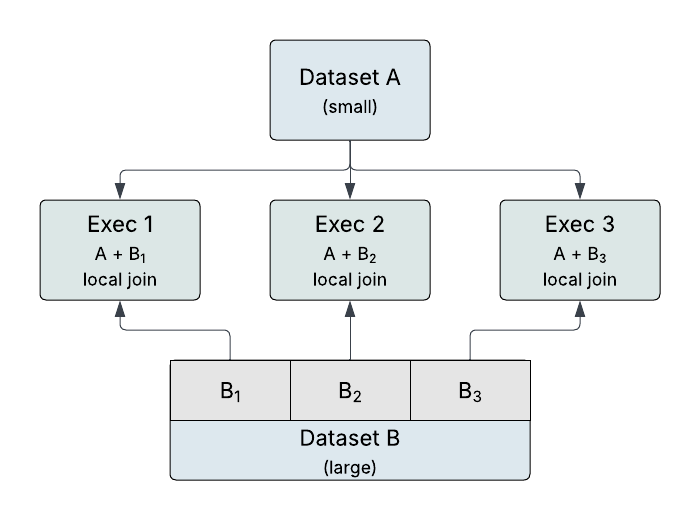
\includegraphics[valign=t, width=0.45\textwidth]{Chapters/02-background/sub-chapters/figures/02-broadcast-join.png}%
% 	}
% 	\hfill
% 	\subfloat[Partitioned join.\label{fig:partitioned-join}]{%
% 		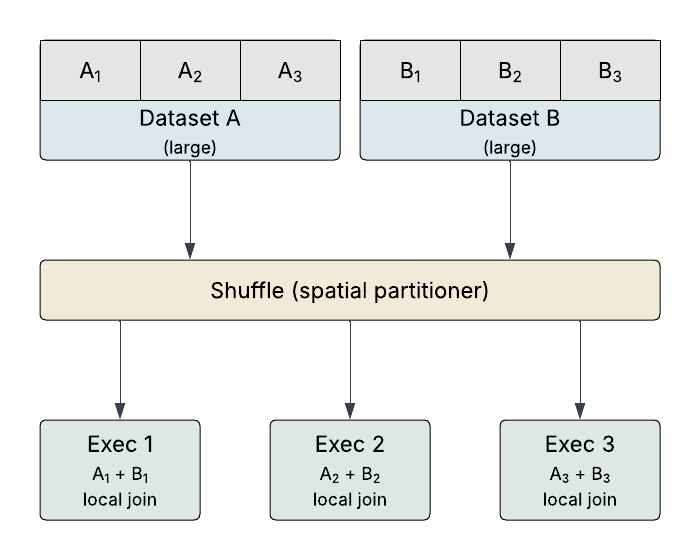
\includegraphics[valign=t, width=0.45\textwidth]{Chapters/02-background/sub-chapters/figures/02-partitioned-join.png}%
% 	}
% 	\caption[Broadcast versus partitioned spatial join]{Broadcast versus partitioned spatial join on the same two inputs. Both strategies converge on the same end state, three executors each performing a local join, but they differ sharply in where the network cost falls. (a) Broadcast: the small input A is shipped from a single source down to every executor; B's partitions are already resident on the executors and do not move, so network traffic scales only with the size of A. (b) Partitioned: both A and B flow through a shuffle that applies a common spatial partitioner, so spatially matching cells of A and B co-locate on each executor before the local join runs. Both inputs traverse the network in this case, and the heavy traffic is the cost of guaranteeing co-location.}
% 	\label{fig:broadcast-vs-partitioned-join}
% \end{figure}

\subsection{Distributed spatial operations}
\label{background:distributed-spatial-processing:distributed-spatial-operations}

Two spatial operations exercise the lifecycle of Section \ref{background:distributed-spatial-processing:the-lifecycle-of-a-distributed-spatial-query} in sharply different ways. The spatial range query filters one input against a fixed query window. The spatial join evaluates a spatial predicate, a boolean condition over geometries, between two inputs.

A spatial range query returns all geometries from an input that lie within a fixed query window \parencite{yu2019_geospark_perspective_beyond}. It runs entirely within a single stage, with each partition filtering its own contents independently of other executors \parencite{yu2019_geospark_perspective_beyond}. Any optimization that reduces the number of partitions scanned therefore translates directly into run-time improvement. File-level bounding-box metadata in GeoParquet supplies one such optimization, allowing the engine to skip files whose extent does not overlap the query window \parencite{sedona2024_geoparquet_loader}. A range query is the operation where a distributed engine is hardest to distinguish from a single-node engine reading the same files, because the work decomposes naturally across files regardless of the partitioner.

The spatial join is the operation where distribution either pays off or breaks down. A spatial join combines two inputs using a spatial predicate, such as intersection or distance, returning the records from each input that satisfy it \parencite{yu2019_geospark_perspective_beyond}. Because records from different executors must be brought together for comparison, the join is a wide operation, one that requires inputs from multiple partitions and therefore crosses a stage boundary \parencite{yu2019_geospark_perspective_beyond}. Two execution strategies have emerged to handle it. In a \emph{broadcast} join, named for the pattern of sending a complete copy of the smaller input to every partition of the larger input, each executor performs a local join against its own partition \parencite{yu2019_geospark_perspective_beyond}. The strict shuffle cost is low, because the engine performs no key-based redistribution, the standard shuffle pattern that hashes or sorts records on a key column to group them across executors. Broadcasting the smaller input nonetheless incurs network traffic that grows with its size. In a \emph{partitioned} join, both inputs are repartitioned by a common spatial partitioner so that records that could possibly satisfy the predicate land on the same executor, and each executor then performs a local join within its own partition without further communication \parencite{yu2019_geospark_perspective_beyond}. Sedona supports KDB-Tree, Quad-Tree, and R-Tree partitioners for this strategy, with the requirement that both inputs be partitioned the same way \parencite{sedona2024_spatial_rdd_application}. Because a polygon may straddle partition boundaries, such records are duplicated into every overlapping partition to preserve correctness, and the system resolves the duplicates after the local join \parencite{yu2019_geospark_perspective_beyond}. The choice between broadcast and partitioned execution is a major lever on the run-time of a distributed spatial workload: a query that switches strategy at a size threshold will exhibit a discontinuous jump in runtime around that threshold. Figure \ref{fig:broadcast-vs-partitioned-join} contrasts the two strategies on the same pair of inputs.

\begin{figure}[H]
	\centering
	\subfloat[Broadcast join.\label{fig:broadcast-join}]{%
		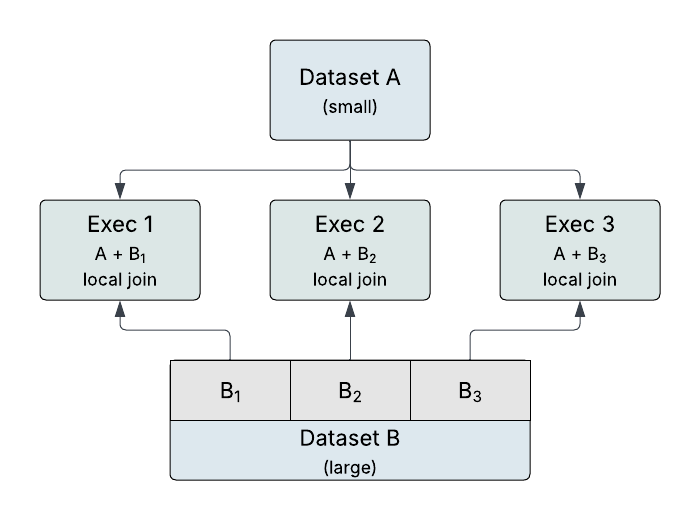
\includegraphics[valign=t, width=0.45\textwidth]{Chapters/02-background/sub-chapters/figures/02-broadcast-join.png}%
	}
	\hfill
	\subfloat[Partitioned join.\label{fig:partitioned-join}]{%
		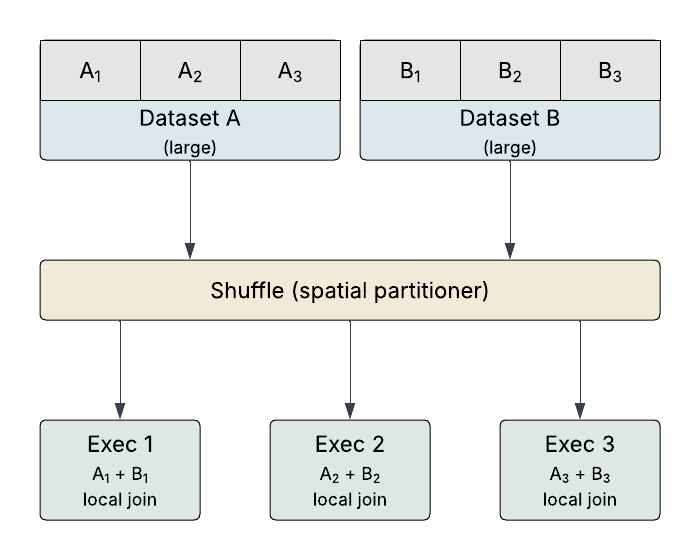
\includegraphics[valign=t, width=0.45\textwidth]{Chapters/02-background/sub-chapters/figures/02-partitioned-join.png}%
	}
	\caption[Broadcast versus partitioned spatial join]{Broadcast versus partitioned spatial join on the same two inputs. Both strategies converge on the same end state, three executors each performing a local join, but they differ sharply in where the network cost falls. (a) Broadcast: the small input A is shipped from a single source down to every executor; B's partitions are already resident on the executors and do not move, so network traffic scales only with the size of A. (b) Partitioned: both A and B flow through a shuffle that applies a common spatial partitioner, so spatially matching cells of A and B co-locate on each executor before the local join runs. Both inputs traverse the network in this case, and the heavy traffic is the cost of guaranteeing co-location.}
	\label{fig:broadcast-vs-partitioned-join}
\end{figure}

% \subsection{Apache Sedona}
% \label{subsec:sedona}
% Apache Sedona, formerly GeoSpark, is an open-source implementation of the spatial extensions described above. \textcite{yu2015_geospark_cluster_computing} introduced it as a Spark extension built around a new abstraction, the \acrfull{srdd}. The system matured through subsequent GeoSpark work, culminating in the comprehensive GeoInformatica reference description by \textcite{yu2019_geospark_perspective_beyond}. SpatialHadoop established this layered design on MapReduce, adding a spatial type system and operators to the distributed engine \parencite{eldawy2015_spatialhadoop_mapreduce_spatial}. Sedona adopts the same structure on Spark, exploiting Spark's in-memory data sharing across operations \parencite{zaharia2012_resilient_distributed_datasets}.

% First, it adds a user-defined Geometry type to Spark \acrshort{sql} \parencite{sedona2024_spatial_sql_application}. Second, it provides a library of spatial functions, exposing functions such as \texttt{ST\_Contains}, \texttt{ST\_Intersects}, and \texttt{ST\_GeomFromWKT} \parencite{sedona2024_spatial_sql_application}. Third, it implements the spatial partitioners and per-partition indexes discussed in Section \ref{background:distributed-spatial-processing:spatial-partitioning-and-parallel-efficiency}, supporting KDB-Tree, Quad-Tree, and R-Tree partitioning together with Quad-Tree and R-Tree local indexes \parencite{sedona2024_spatial_rdd_application}. Fourth, it integrates with Catalyst \parencite{yu2019_geospark_perspective_beyond}, making these capabilities available through both the \acrshort{srdd} \acrshort{api} and the higher-level Sedona \acrshort{sql}/DataFrame \acrshort{api} \parencite{sedona2024_spatial_rdd_application,sedona2024_spatial_sql_application}. Figure \ref{fig:sedona-architecture-on-spark} situates these four features within Sedona's layered design over Spark Core.

% \begin{figure}[H]
% 	\centering
% 	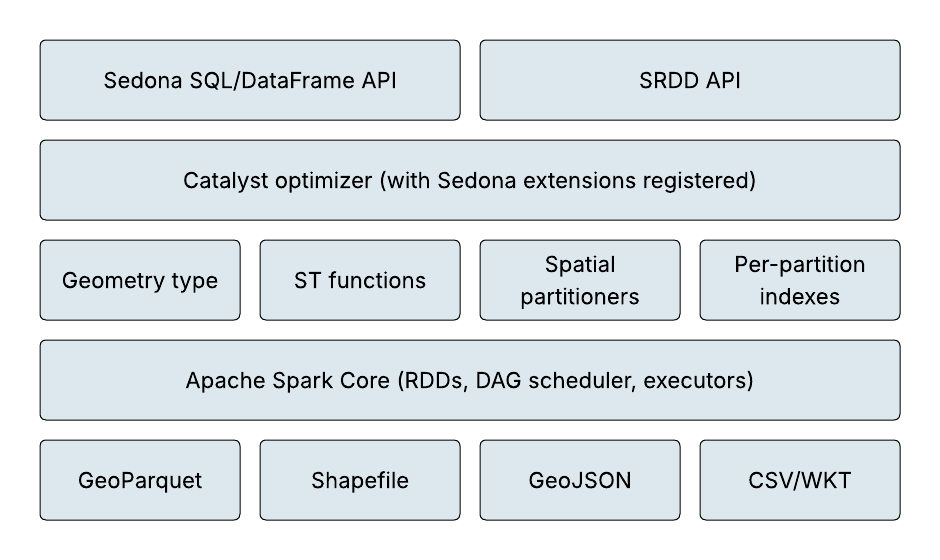
\includegraphics[width=0.7\textwidth]{Chapters/02-background/sub-chapters/figures/02-sedona-architecture-on-spark.png}
% 	\caption[Apache Sedona architecture on Apache Spark]{Layered architecture of Apache Sedona on Apache Spark. From top to bottom: two user-facing APIs (Sedona SQL/DataFrame and SRDD); the Catalyst optimizer with Sedona's \acrlong{udf}s~(\acrshort{udf}) and types registered; the four spatial extensions enumerated in the surrounding paragraph (Geometry type, ST functions, spatial partitioners, per-partition indexes); the Apache Spark runtime; and the storage formats Sedona reads directly. Adapted from \parencite{yu2015_geospark_cluster_computing}.}
% 	\label{fig:sedona-architecture-on-spark}
% \end{figure}

% Direct GeoParquet support is the feature that makes Sedona a suitable point of comparison for cloud-native query engines. Sedona reads the per-file bounding-box metadata defined by the GeoParquet specification and uses it to discard files whose extent cannot satisfy a spatial predicate, reducing the number of files scanned when the dataset is partitioned by spatial proximity \parencite{sedona2024_geoparquet_loader}. The combination of \acrshort{srdd}s, ST functions, spatial partitioners, and GeoParquet readers makes Sedona directly comparable to DuckDB on GeoParquet at the data-format level, while the underlying Spark run-time supplies the distributed lifecycle described in Section \ref{background:distributed-spatial-processing:the-lifecycle-of-a-distributed-spatial-query}.

\subsection{Apache Sedona}
\label{background:distributed-spatial-processing:apache-sedona}
Apache Sedona, formerly GeoSpark, is an open-source library that realizes the spatial extensions discussed in the preceding subsections on Apache Spark. \textcite{yu2015_geospark_cluster_computing} introduced it as a Spark extension built around a new abstraction, the \acrfull{srdd}, and later GeoSpark work consolidated the design in the GeoInformatica reference description by \textcite{yu2019_geospark_perspective_beyond}. The same layered design appeared earlier in SpatialHadoop, an analogous extension that added a spatial type system and operators to the Hadoop MapReduce engine, the batch-parallel paradigm that preceded Spark \parencite{eldawy2015_spatialhadoop_mapreduce_spatial}. Sedona adopts that structure on Spark and exploits Spark's in-memory data sharing across operations \parencite{zaharia2012_resilient_distributed_datasets}.

Sedona contributes four spatial extensions to the Spark engine. First, it adds a user-defined Geometry type to Spark \acrshort{sql} \parencite{sedona2024_spatial_sql_application}. Second, it provides a library of spatial functions, including \texttt{ST\_Contains}, \texttt{ST\_Intersects}, and \texttt{ST\_GeomFromWKT} \parencite{sedona2024_spatial_sql_application}. Third, it implements the spatial partitioners and per-partition indexes discussed in Section \ref{background:distributed-spatial-processing:spatial-partitioning-and-parallel-efficiency}, supporting KDB-Tree, Quad-Tree, and R-Tree partitioning together with Quad-Tree and R-Tree local indexes \parencite{sedona2024_spatial_rdd_application}. Fourth, it integrates with Catalyst \parencite{yu2019_geospark_perspective_beyond}, exposing these capabilities through both the \acrshort{srdd} \acrshort{api} and the higher-level Sedona \acrshort{sql}/DataFrame \acrshort{api} \parencite{sedona2024_spatial_rdd_application,sedona2024_spatial_sql_application}. Figure \ref{fig:sedona-architecture-on-spark} situates these four features within Sedona's layered design over Spark Core.

\begin{figure}[H]
	\centering
	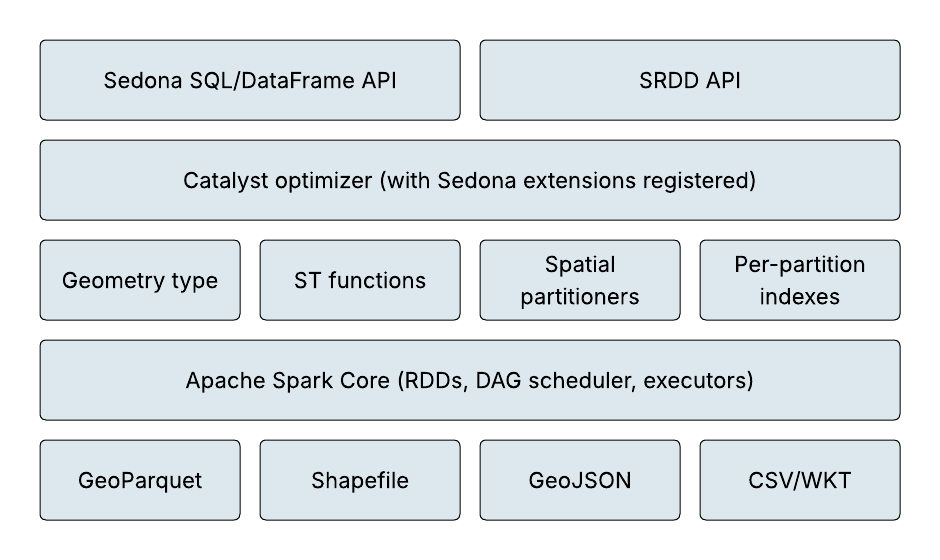
\includegraphics[width=0.7\textwidth]{Chapters/02-background/sub-chapters/figures/02-sedona-architecture-on-spark.png}
	\caption[Apache Sedona architecture on Apache Spark]{Layered architecture of Apache Sedona on Apache Spark. From top to bottom: two user-facing APIs (Sedona SQL/DataFrame and SRDD); the Catalyst optimizer with Sedona's \acrlong{udf}s~(\acrshort{udf}) and types registered; the four spatial extensions enumerated in the surrounding paragraph (Geometry type, ST functions, spatial partitioners, per-partition indexes); the Apache Spark runtime; and the storage formats Sedona reads directly. Adapted from \parencite{yu2015_geospark_cluster_computing}.}
	\label{fig:sedona-architecture-on-spark}
\end{figure}

Direct GeoParquet support is the feature that makes Sedona a suitable point of comparison for cloud-native query engines. Sedona reads the per-file bounding-box metadata defined by the GeoParquet specification and uses it to discard files whose extent cannot satisfy a spatial predicate, reducing the number of files scanned when the dataset is partitioned by spatial proximity \parencite{sedona2024_geoparquet_loader}. The combination of \acrshort{srdd}s, ST functions, spatial partitioners, and GeoParquet readers makes Sedona directly comparable to DuckDB on GeoParquet at the data-format level, while the underlying Spark run-time supplies the distributed lifecycle described in Section \ref{background:distributed-spatial-processing:the-lifecycle-of-a-distributed-spatial-query}.

% \subsection{Databricks as a Sedona run-time}
% \label{subsec:databricks}
% Apache Sedona is a library, not a managed service: it extends Apache Spark with distributed spatial datasets and functions, and therefore runs only inside an existing Spark cluster \parencite{sedona2026_sedonaspark}. Several run-time properties of the Databricks-managed Spark platform shape how a Sedona job behaves on Azure, independently of Sedona itself, and matter when interpreting elapsed time and cost on this platform. Four such properties together determine the cost of a Sedona run beyond the cost of the query itself: cluster startup, autoscaling, the separation of compute from storage, and node-hour billing.

% A Databricks cluster consists of a driver node and zero or more worker nodes, each backed by a cloud-provider VM that must be acquired and initialized before any task runs \parencite{databricks2024_compute_configuration}. Databricks documents that classic compute has longer startup times than serverless \parencite{databricks2024_cost_optimization_best_practices}, during which the cloud provider bills for the underlying VMs even when no workload is running \parencite{databricks2024_pool_index}. For short queries, this provisioning interval can dominate wall-clock time \parencite{databricks2024_cost_optimization_best_practices}.

% Autoscaling controls the number of executors actively billed during a job \parencite{databricks2024_compute_configuration}. Databricks's optimized autoscaler tracks idle executors and removes them when work has drained, even mid-job \parencite{databricks2018_optimized_autoscaling}. Autoscaling decisions are made at a polling interval \parencite{databricks2024_compute_configuration}, so a burst of work that completes within that interval will not see additional executors provisioned. As a result, two runs of the same query on the same nominal cluster configuration can encounter different effective parallelism depending on whether the autoscaler has settled \parencite{databricks2018_optimized_autoscaling, databricks2024_compute_configuration}.

% A Databricks cluster reads data from external object storage over the network rather than from cluster-local disks~\parencite{databricks2025_lakehouse, pang2024_storage_disaggregated_databases}. Every cold read therefore crosses the network between compute and storage \parencite{pang2024_storage_disaggregated_databases}, and that cost is absorbed into the executor read time described in Section \ref{background:distributed-spatial-processing:the-lifecycle-of-a-distributed-spatial-query}.

% Databricks bills compute at per-second granularity~\parencite{databricks2024_pricing}. The cost of a Sedona run is therefore the product of the cluster size and its lifetime, including provisioning~\parencite{databricks2024_pool_index} and any post-job idle period before auto-termination~\parencite{databricks2024_compute_configuration}. The relationship between elapsed query time and billed compute time on this platform is therefore mediated by these run-time properties rather than determined by the query alone.

\subsection{Databricks as a Sedona run-time}
\label{background:distributed-spatial-processing:databricks-as-a-sedona-run-time}
Apache Sedona is a library rather than a managed service, extending Apache Spark with distributed spatial datasets and functions, and therefore runs only inside an existing Spark cluster \parencite{sedona2026_sedonaspark}. On Azure, Databricks, a managed Apache Spark service, supplies that cluster, and several run-time properties of the platform shape how a Sedona job behaves independently of Sedona itself, which matters when interpreting elapsed time and cost. Four such properties together determine the cost of a Sedona run beyond the cost of the query itself: cluster startup, autoscaling, the separation of compute from storage, and node-hour billing.

A Databricks cluster consists of a driver node and zero or more worker nodes, each backed by a cloud-provider \acrfull{vm}, a software-emulated computer the provider allocates from physical hardware, that must be acquired and initialized before any task runs \parencite{databricks2024_compute_configuration}. Databricks documents that classic compute, the non-serverless cluster mode in which the customer specifies the \acrshort{vm} type and count, has longer startup times than serverless \parencite{databricks2024_cost_optimization_best_practices}, during which the provider bills for the underlying \acrshort{vm}s even when no workload is running \parencite{databricks2024_pool_index}. For short queries, this provisioning interval can dominate wall-clock time \parencite{databricks2024_cost_optimization_best_practices}.

Autoscaling controls the number of executors actively billed during a job \parencite{databricks2024_compute_configuration}. Databricks's optimized autoscaler tracks idle executors and removes them when work has drained, even mid-job \parencite{databricks2018_optimized_autoscaling}. Decisions are made at a polling interval, a fixed cadence at which the autoscaler reassesses cluster load \parencite{databricks2024_compute_configuration}, so a burst of work that completes within that interval will not see additional executors provisioned. Two runs of the same query on the same nominal cluster configuration can therefore encounter different effective parallelism depending on whether the autoscaler has settled \parencite{databricks2018_optimized_autoscaling, databricks2024_compute_configuration}.

A Databricks cluster reads data from external object storage over the network rather than from cluster-local disks \parencite{databricks2025_lakehouse, pang2024_storage_disaggregated_databases}. Every cold read, a read against data not already cached on the executor, therefore crosses the network between compute and storage \parencite{pang2024_storage_disaggregated_databases}, and that cost is absorbed into the executor read time described in Section \ref{background:distributed-spatial-processing:the-lifecycle-of-a-distributed-spatial-query}.

Databricks bills compute at per-second granularity \parencite{databricks2024_pricing}. The cost of a Sedona run is the product of cluster size and lifetime, including the provisioning interval \parencite{databricks2024_pool_index} and any post-job idle period before auto-termination \parencite{databricks2024_compute_configuration}. Elapsed query time and billed compute time on this platform are therefore mediated by these run-time properties rather than determined by the query alone.

% \subsection{Summary}
% \label{subsec:dist-summary}
% A distributed spatial query follows a fixed lifecycle: driver-side planning, parallel reads from object storage, narrow stages pipelined within executors, wide stages separated by shuffles, and a final action that writes results or collects them on the driver. Whether this lifecycle parallelizes depends on a spatial partitioner that co-locates nearby geometries, a per-partition local index that accelerates the local work, and the absence of skew that would funnel work onto a single straggler. Range queries run within a single stage, while spatial joins cross a stage boundary and are resolved via either broadcast or partitioned execution. Apache Sedona provides the spatial types, functions, partitioners, and GeoParquet readers needed to express these operations as Spark \acrshort{sql} queries, while Databricks provides the cluster lifecycle, autoscaling, and object storage connectivity that make Sedona a running service.

\subsection{Summary}
\label{background:distributed-spatial-processing:summary}
A distributed spatial query follows a fixed lifecycle: driver-side planning, parallel reads from object storage, narrow stages pipelined within executors, wide stages separated by shuffles, and a final action that writes results or collects them on the driver. The lifecycle parallelizes only when three conditions hold: a spatial partitioner co-locates nearby geometries, a per-partition local index accelerates the work within each partition, and skew does not funnel work onto a single straggler. Range queries run within a single stage; spatial joins cross a stage boundary and resolve through either broadcast or partitioned execution. Apache Sedona supplies the spatial types, functions, partitioners, and GeoParquet readers that express these operations as Spark \acrshort{sql} queries. Databricks supplies the cluster lifecycle, autoscaling, and object storage connectivity that make Sedona a running service.